\section{Francesco}\label{sec:francesco}

% Encoding and language

\newenvironment{cverbatim}
  {\begin{center}\begin{minipage}{0.7\linewidth}\begin{verbatim}}
  {\end{verbatim}\end{minipage}\end{center}}

\nocite{*}
\section{Section 1 -- Nucleo-F411RE/U545RE (MCU)}


For the development of the required model, a microcontroller is needed that can help with the debug of the various trial versions. The most used model in the literature is the following:
\begin{center}
    Nucleo-F411RE
\end{center}
This is the STM32F411 version with more Flash and Ram, especially suitable for development. There is a Micro-USB connector to connect it to the PC and therefore to the handy IDE called STM32CubeIDE. The project is then created and the .tflite model is loaded inside the IDE which facilitates compilation and adaptation with the specific commands. Once the project is working, the use of the smaller and more performing F411CEU6 ‘Black Pill’ or equivalent will be preferred.

\subsection{Introduction}

First of all, it is possible to download the IDE from the official site, and the installation is rather simple on debian-based Linux machines. It is sufficient to run the .sh installer with sudo permissions and, for now, deny the installation of plugins for non-Nucleo boards.

At this point, we create a new project: File $\rightarrow$ New $\rightarrow$ STM32 Project. Then, click on the Board Selector tab $\rightarrow$ Nucleo-F411RE + next $\rightarrow$ leave HAL as library, Toolchain/IDE = STM32CubeIDE $\rightarrow$ Finish

There will be a warning indicating that the firmware package for the F411x series is not installed. We will therefore be forced to create an account on STM and, having done so, in the project Help $\rightarrow$ Updates $\rightarrow$ Connection to myST

At this point, still on Help $\rightarrow$ Conf tools $\rightarrow$ Manage … $\rightarrow$ STM32Cube MCU Package for STM32F4 Series (STM32CubeF4). $\rightarrow$ Install {~ 1 Gb}

\begin{table}[h]
\centering
\begin{tabular}{l l l l}
    oprule
Package & Installed version & Available version & Size \\
\midrule
MCU Package for STM32F4 Series & 1.28.3 & 1.28.3 & -- \\
MCU Package for STM32F4 Series & --     & 1.28.2 & 925.0 MB \\
MCU Package for STM32F4 Series & --     & 1.28.1 & 895.0 MB \\
\bottomrule
\end{tabular}
\caption{STM32Cube MCU Packages (extract)}
\end{table}

\subsection{A quick look at the architecture}

\begin{figure}[h]
\centering
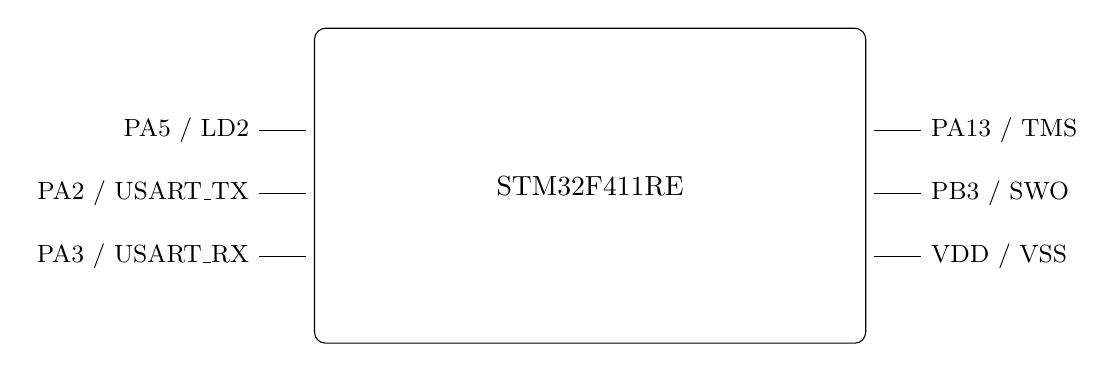
\begin{tikzpicture}[
    pinlabel/.style={font=\small},
    >=stealth
]
\node[draw, rounded corners, minimum width=7cm, minimum height=4cm, align=center] (mcu)
    {STM32F411RE};

% Left side
\node[pinlabel, anchor=east] (pa5)  at ([xshift=-0.7cm,yshift=0.7cm]mcu.west) {PA5 / LD2};
\node[pinlabel, anchor=east] (pa2)  at ([xshift=-0.7cm,yshift=-0.1cm]mcu.west) {PA2 / USART\_TX};
\node[pinlabel, anchor=east] (pa3)  at ([xshift=-0.7cm,yshift=-0.9cm]mcu.west) {PA3 / USART\_RX};

\draw (pa5.east) -- ([xshift=-0.1cm]mcu.west |- pa5.east);
\draw (pa2.east) -- ([xshift=-0.1cm]mcu.west |- pa2.east);
\draw (pa3.east) -- ([xshift=-0.1cm]mcu.west |- pa3.east);

% Right side
\node[pinlabel, anchor=west] (pa13) at ([xshift=0.7cm,yshift=0.7cm]mcu.east) {PA13 / TMS};
\node[pinlabel, anchor=west] (pb3)  at ([xshift=0.7cm,yshift=-0.1cm]mcu.east) {PB3 / SWO};
\node[pinlabel, anchor=west] (vdd)  at ([xshift=0.7cm,yshift=-0.9cm]mcu.east) {VDD / VSS};

\draw ([xshift=0.1cm]mcu.east |- pa13.west) -- (pa13.west);
\draw ([xshift=0.1cm]mcu.east |- pb3.west)  -- (pb3.west);
\draw ([xshift=0.1cm]mcu.east |- vdd.west)  -- (vdd.west);
\end{tikzpicture}
\end{figure}

The board has a main microcontroller with CPU, RAM and FLASH memory. In addition, various buses are available on it, including
\begin{itemize}
    \item $I^2C$: 2-wire bus (SCL clock, SDA data) on which several sensors can be connected and each has an address. E.g. the CPU asks sensor 0x68 for 6 bytes starting from 0x00 $\rightarrow$ they are passed on SDA at SCL rate.
    \item UART: two much simpler wires (TX send, RX receive), used for log/test between PC and Board in debug. The CPU buffers in internal RAM every data that arrives on RX. Naturally asynchronous, it can also be set to synchronous (USART).
\end{itemize}
It should also be remembered the \textbf{NVIC} interface inside the CPU which manages incoming interrupts (for example from GPIO) and delegates specific callbacks for its handling.

In addition to the primary chip, there is a secondary \textbf{ST-LINK} smaller, near the micro-USB connector, which acts as a bridge with the PC and the Board. It has a converter called Virtual COM to make USB – USART communication possible and therefore fundamental to connect PC and board. This chip is used to program the firmware inside the primary and for the various debug (pause, breakpoints, lookup variables in CubeIDE). Example of operation:
\begin{itemize}
    \item Programming: when I want to load the file compiled from PC onto the F411 chip, it is first sent to ST-LINK which through a special serial interface SWD (not the USART one) writes those bytes in FLASH of the main microcontroller through two specific pins. The latter will take care of execution.
    \item Debug: the same SWD interface is used to stop execution, set breakpoints or read registers/RAM $\rightarrow$ full control
    \item Log: through the Virtual COM bridge, as said before, it allows communication through TX/RX. In particular, every printf() in the code is written on TX and therefore received by the PC via COM.
\end{itemize}

\subsubsection{Some tests}
The initial interface is that of the ‘\textit{designer}’ (.ioc) file. The first action to be carried out is to activate the buses mentioned above: Connectivity $\rightarrow$ I2C1 $\rightarrow$ $I^2C$ 

At this point the CPU pins will light up green (they can be changed if desired). In any case, from the ‘Parameter Settings’ screen at the bottom it is convenient to activate the Fast Mode in Master Features. 

Now we will activate \textbf{UART} (usually by default) leaving async instead of sync and leaving the configuration 115200 bit/s 8 bit/words 1 Stop bit (every word ends with a bit at 1). This is the standard of any serial terminal required by default for communication with PC. 

We just have to \textit{scan the sampling time} equal to 1Hz: Timers $\rightarrow$ TIM2 $\rightarrow$ ‘Clock Source’ = Internal Clock. Now it is necessary to open the Clock configuration tab, which will expose all the clocks of each part of the board (e.g. Ethernet, Cortex, Peripherals…). What interests us is APB1 and APB1x2, the slower paths for the peripherals, which have prescalers to divide the clock (depower it). For this reason, it is necessary to note down the two APB1 values, return to Pinout configuration and configure Prescaler-CounterPeriod following the \textit{formula}: 

\begin{equation}
f_{\text{update}} = \frac{f_{\mathrm{TIMxCLK}}}{(PSC + 1)\,(ARR + 1)} \, .
\end{equation}

Since the clock on APB1 is 42Mhz, we will set prescaler equal to 8399 and Counter Period 9999 (both with the -1 due to the +1 in the formula). We will therefore use TIM2 as timer for our model. Also check ‘enabled’ in NVIC Settings to allow the timer to send an \textbf{interrupt} at each Hz to the CPU via NVIC. 

\begin{table}[h]
\centering
\begin{tabular}{l l}
\toprule
Setting          & Value \\
\midrule
Prescaler (PSC - 1)   & 8399 \\
Counter Mode          & Up \\
Counter Period (ARR)  & 9999 \\
Internal Clock Division & No Division \\
Auto-reload preload   & Disable \\
\bottomrule
\end{tabular}
\end{table}

\begin{table}[h]
\centering
\begin{tabular}{l c c}
\toprule
Interrupt           & Enabled & Preemption Priority \\
\midrule
TIM2 global interrupt & \checkmark & 0 \\
\bottomrule
\end{tabular}
\end{table}

\subsubsection{Organization of the main.c file }

First of all, the file is divided into 3 main parts:
\begin{itemize}
    \item Preliminary operations: includes, static functions and global variables.
    \item Main: Initializes the main functionalities, including HAL, Clock and in our case it must start the Timer (ready for interrupt). Finally, it continues with a while(1) loop that includes the logic to follow during work.
    \item Callbacks and more: Here timers and possible Hardware redirection functions are created. For example, we will extend a system callback that is called at every timer NVIC Interrupt and, through specific selection for that timer, we will do a Toggle.
\end{itemize}

For experimental reasons, it was decided to suspend the development on the much used and simple F411RE to move towards a more cutting-edge MCU: the U series in fact, are much more recent boards: the little documentation available and, above all, the interface in the IDE (much more rudimentary) bear witness to this. Let us see some key features of the
\begin{center}
    \textit{Nucleo-U545RE}
\end{center}

\begin{itemize}
    \item Cortex-M33 at 160 MHz: faster than the previous 100MHz
    \item Flash 2MB, RAM 786KB. Both 4 times compared to the F411RE
    \item New connectivity: USB C (double, one also for direct loading without STLINK), I3C, advanced Timers for modern sensors, ...
    \item Reduced consumption: The processor is at 40nm instead of 90, therefore smaller and faster transistors with less energy dissipation at the same frequency.
\end{itemize}

Finally, the U5 series is specifically designed for the minimum indispensable consumption: in addition to the classic run/sleep/standby there are other \textit{energy saving} modes available. There is also a clock source Multi Speed Internal Oscillator MSIS which is specifically designed to operate in ultra low power.

\subsection{Initial setup}

Set the clock \textit{high} just to become familiar with the diagram of the internal sources.

Starting from the left, we observe that there are 2 types of sources that interest us: HSI-RC and MSIS. They end up towards the right in the System Clock Multiplexer. By default, this Mux selects \textbf{MSIS}. We want HSI-RC (which starts from 16MHz, but has dividers and multipliers to adjust it exactly to our need, unlike MSIS, difficult to drive).

We therefore set Mux to \textbf{PLLCLK} (it comes from HSI, to be selected in the PLL1 Source Multiplexer) and adjust the corresponding M/D to get to \textbf{160MHz} using simple \textit{logical} reasoning. Let us finally make sure that the APB outputs of the peripherals are also at 160MHz.

We are thus ready to proceed with the creation of the timer + interrupt handler, continuing with our test project. Obviously, if the clock overflows (maximum allowed CLK 160MHz) an error in purple is shown.

\subsection{Interrupt handling on LED toggle}

First go to Pinout-Configuration $\rightarrow$ Click pin Pa5(LED) $\rightarrow$ Select GPIO\_Output $\rightarrow$ by doing a \textit{toggle}, it will alternate at 1Hz if everything is correct. 
During the saving of the project or closing, the IDE will ask if you want to \textbf{generate} the associated code. Answer yes or, otherwise, generate it at a later time: Project $\rightarrow$ Generate Code (gear icon). Now open Core/Src/main.c $\rightarrow$ there will be all the modules that are initialized, including:

\begin{verbatim}
MX_GPIO_Init();
MX_USART2_UART_Init();
MX_I2C1_Init();
MX_TIM2_Init();
\end{verbatim}

We notice that what we have talked about so far is initialized; however, TIM2 (timer) does not start by itself: it needs a start function to be inserted immediately afterwards:

\begin{verbatim}
HAL_TIM_Base_Start_IT(&htim2);
\end{verbatim}

At this point, at each tick its callback is called. Outside the main, the callback must be composed as follows:

\begin{lstlisting}[language=C]
/* USER CODE BEGIN 4 */
void HAL_TIM_PeriodElapsedCallback(TIM_HandleTypeDef *htim)
{
    if (htim->Instance == TIM2) {
        HAL_GPIO_TogglePin(GPIOA, GPIO_PIN_5);  // LED blink
        printf("tick\r\n");                     // message on Virtual COM
    }
}
/* USER CODE END 4 */
\end{lstlisting}

I will therefore expect a toggle every second and a printf on PC (through Virtual COM) that writes `tick`. 

An extension is therefore added at low level just before the callback. Normally, on a PC the printf() is sent to the default terminal. Unfortunately, it is not so simple here: STM32 does not have a real virtual terminal, and no OS. Recalling that in C (Linux): 
printf calls the system call write() --> system trap --> kernel --> terminal. We will have to simulate the same behaviour. Here, printf calls \_write() which calls \_\_io\_putchar, which will be extended to write on the UART/USART previously activated.

% __io_putchar with USART2
\begin{lstlisting}[language=C]
int __io_putchar(int ch) {
    HAL_UART_Transmit(&huart2, (uint8_t *)&ch, 1, 10);
    return ch;
}
\end{lstlisting}

\subsubsection{Very important note}

In this first test project optimizations are not the main topic, we reason from a purely \textit{didactic} point of view. In reality, one must be very careful with printf operations and, more generally, with the hardware side.
In particular, when the callback is called, one should \textbf{never} write a printf inside it. this is because interrupts block by definition the other interrupts of the same or higher level, and therefore with a more or less long operation (e.g. printf) one risks \textit{losing other} urgent interrupts or incoming data. For this reason, it is convenient:

\begin{itemize}
    \item Avoid printing inside the callback by adding only a flag update.
    \item In the while(1) of the main, print every time the flag changes and then re-initialize it.
\end{itemize}

In this way, the CPU is interrupted for a very short time and, despite finishing the interrupt handling tasks, remains listening.
In our case, a possible solution could therefore be to declare the tick flag (always in section 4, above \_\_io\_putchar):

\begin{verbatim}
volatile uint8_t tick_flag = 0;
\end{verbatim}

Then change the Callback function:

\begin{lstlisting}[language=C]
void HAL_TIM_PeriodElapsedCallback(TIM_HandleTypeDef *htim)
{
    if (htim->Instance == TIM2) {
        HAL_GPIO_TogglePin(GPIOA, GPIO_PIN_5);  // LED blink
        tick_flag = 1;                          // signal
    }
}
\end{lstlisting}

Finally, modify the while(1) of the main for the management of the print (or other f):

\begin{lstlisting}[language=C]
/* USER CODE BEGIN WHILE */
while (1)
{
    /* USER CODE BEGIN 3 */
    if (tick_flag) {
        tick_flag = 0;
        printf("tick\r\n");
    }
    /* USER CODE END 3 */
}
/* USER CODE END WHILE */
\end{lstlisting}

Having said this, it remains the fact that we are using an AI model and we are not obliged to the hard-realtime constraint: latency can be \textit{tolerated}.

% =========================
\subsubsection{Virtual COM serial visualization}
At this point everything is ready: we only need to be able to display the \textbf{serial} output on our PC. Install the program \textit{screen}:
\begin{verbatim}
sudo apt install screen
\end{verbatim}
Search for the associated dev file (typically ACM driver):
\begin{verbatim}
sudo dmesg | grep tty
\end{verbatim}
Display the terminal (it will print 'tick' every N ms):
\begin{verbatim}
screen /dev/ttyACM0 115200
\end{verbatim}

To exit: Ctrl+A -> \textbackslash{} -> Y. 

% dmesg: recognition of the ttyACM0 device
\begin{lstlisting}[language=bash]
[344455.760043] cdc_acm 3-1.4:1.2: ttyACM0: USB ACM device
[350968.094608] cdc_acm 3-1.4:1.2: ttyACM0: USB ACM device
\end{lstlisting}


% Output of the serial with the ticks
\begin{lstlisting}[language=bash]
tick
tick
tick
tick
tick
tick
...
\end{lstlisting}

\subsubsection{Notes}
The number 115200 is the default baud left on USART1.

\subsection{Test of import of CNN-only model}
First of all, actually \textbf{the board visualization plugin is available.} The important thing is to choose the only one with the entry board among those that show the same acronym \textbf{U545RE}.

We therefore proceed to a test project in which we will try to \textit{import a model} (CNN only, for now) into the MCU. There will be some steps not entirely correct initially, and for this reason note that the guide follows the \textit{numerous attempts} and is not rewritten only on the basis of the working parts

\subsubsection{From float32 to int8}
In this test project, we will become familiar converting a model into TensorflowLiteMicro, and then import it with all the tools necessary for optimal operation. It should be specified that, for now, we have not yet chosen a model to use \textit{by default}. Therefore, a simple test CNN model on the sampled data (No LSTM) will be used, converted through TFlite Micro \textbf{without optimizing, for now}.

\begin{center}
    \textit{Use a classic python converter script}
\end{center}


Note: an error will probably be shown due to the training that contains the evaluation and other data. This fact can be \textit{ignored} by modifying a parameter (compile=False) thus forcing non-recompilation. Note that this fact can be ignored \textbf{if and only if} one plans to mount the model directly for inference. If instead one thinks of having to modify it in its Core (e.g. adding/removing weights in this reduced phase) it will then be vitally important to include the parameter in order not to lose the training data.

\begin{center}
    \textit{This is not our case.}
\end{center}

Once this operation is finished, we are not yet ready for the actual export: in fact, in order to be imported into our project it is necessary to \textit{convert it into an} unsigned char array importable as .h in main.c. We therefore proceed with the command:
\begin{verbatim}
xxd -i modello_int8.tflite > modello_int8.cc
\end{verbatim}
Now everything is ready, we will move on to the IDE.

\subsubsection{Import of the necessary libraries}
Naturally, it is not enough to have the model: it is necessary to install the \textit{Tensorflow lite Micro libraries} in our project so that the code can be correctly interpreted. At this point it is possible to clone Tensorflow and Flatbuffers onto our PC, in any folder. It will then be necessary to copy them inside the project.

After the import, compiler update and headers update, there are a lot of problems and errors. To be brief:
\begin{itemize}
    \item Compiling problem without C++, also after converting it
    \item Missing modules from libraries
    \item GZip compressing 166Gb of logs on 'tick' output terminal before
    \item No U545 Modules without hotspot connection (Firewall problem)
\end{itemize}


\subsection{New path: X-CUBE-AI Plugin}
\subsubsection{Introduction}

The plugin in question has been developed specifically to simplify the use of platforms such as TFlite/Keras on stm32 MCUs. The first operation to be done will therefore be to proceed with the installation and, subsequently, proceed with the \textit{build} of the model on the microcontroller.

\subsubsection{Import of the plugin and of the model}
Navigate in the .ioc file and, under Middleware and Software Packs, find xcubeAI and install the latest version. At this point the \textit{active} plugin will appear and you can click to navigate in its menu. Attention: Click on the plugin, tick Core and select Application Template. \textit{Save}.

At this point, reopen cubeAI, click Add Network --> tflite --> browse --> select the model and confirm. In order to generate the code with the AI logic, it is necessary to \textbf{analyze} the model in advance.

\subsubsection{Important notes}
\begin{itemize}
    \item Clear Pinouts: Clean all the pinouts in case they are previously populated by standard CubeIDE functions: Pinout config $\rightarrow$ Pinout $\rightarrow$ Clear Pinouts
    \item Enable Float: The project will reason with float input/output, despite the microcontroller reasoning in int8. For debug, for now activate floats in printf/scanf : Project $\rightarrow$ Properties $\rightarrow$ C/C++ Build $\rightarrow$ Settings $\rightarrow$ MCU Settings $\rightarrow$ tick “Use float with printf”
    \item Clock At 160MHz: To avoid problems during the transmission of data to and from the outside (with respect to the model) configure the maximum clock to be sure of having enough reasoning speed.
\end{itemize}

\subsubsection{Analysis of the model}
At this point we can proceed with the analysis of the model, before importing it. Select Analyze $\rightarrow$ a classic error will be displayed: the shell cannot be opened here (WISH window shell is needed):

\begin{verbatim}
sudo apt install tcl tk
\end{verbatim}

Tool Command Language is used for \textit{scripting} while Tk (Toolkit) is used for \textit{graphical interfaces} (GUI), including Window Shell). Now it analyzes correctly with output on the IDE shell.

\subsubsection{Compilation and resolution of the warnings.}
We therefore proceed with the compilation and resolution of the warnings. Build $\rightarrow$ Build Project. 

% Extract of the linker warnings in STM32CubeIDE
\begin{lstlisting}[language=bash]
.text._close_r+0x0c): warning: _close is not implemented and will always fail
...
.text._write_r+0x10): warning: _write is not implemented and will always fail
\end{lstlisting}

The .elf file will be correctly generated, but \textit{warnings} will be shown (which the board translates as Error at compilation time) regarding the standard library (newlib-nano), typical when printf() or automatically generated C functions are available and call POSIX system calls (_close, _kill, _lseek, _read, ...).

They do not exist on the microcontroller, and as we have already said they must be redirected. For a more \textit{clean} solution, this time we will implement a file that at compilation time will solve all these problems. Place it in Src and the compiler will take care of the rest. 

\textbf{Note}: Now activate UART1, otherwise the change on the print/scan header cannot be applied. With NVIC Interrupt.

% Minimal syscalls_min.c with retranslation stdout/stderr -> UART1
\begin{lstlisting}[language=C]
// Core/Src/syscalls_min.c
#include ...

extern UART_HandleTypeDef huart1;

// stdout/stderr -> UART1
int _write(int file, char *ptr, int len) {
    if (file == STDOUT_FILENO || file == STDERR_FILENO) {
        HAL_UART_Transmit(&huart1, (uint8_t *)ptr, len, HAL_MAX_DELAY);
        return len;
    }
    errno = EBADF;
    return -1;
}

...

int _read(int file, char *ptr, int len) {
    if (file == STDIN_FILENO) {
        errno = EAGAIN;
        return -1;
    }
    errno = EBADF;
    return -1;
}


}
\end{lstlisting}

Now at each \textbf{run} (that is deployment on the board) the model will be loaded without errors. Note that the run implies loading the model in flash and consequent setup in RAM of the Tensorflow arena. So, everything \textit{automatic}. We will then see the infrastructure that is created during the run and how it reasons, and then manage to interact with it through \textbf{UART}.

\textbf{Final considerations}
\begin{itemize}
    \item Stm32cube ide is not able to convert by itself ad hoc, but only by specifying in the drop-down the 'degree' of \textit{compression} and on which target (RAM or Flash). You can also select a light h5 model in case you have managed to create it and run it pure \textit{as it is}.  
    \item The starting model in h5, for now, weighs only 1Mb. Not realistic. In any case, by quantizing it with the converter [without accuracy, see point 3] it results 1/10 (~100kB) (CNN). Instead LSTM + CNN ~1200kB --> 120kB miniaturized. 
    \item Once the model has been chosen, care must be taken during the conversion: \textbf{the batch of representative dataset} on which to quantize must be chosen carefully (and not random, as now): in fact, when the model is shrunk, one must 'make the model notice' the typical \textbf{range} of input data. In this way those input intervals will be 'eliminated'. To give an example, let us imagine that the typical temperature range is between 30 and 70 degrees. It does not make any sense at all to choose a range including values below zero.
    \item When I say 1/10 I actually mean \textbf{1/3}: practically the model by going on properties from the file system we see that it weighs 1Mb, but in reality the non-removable part in deployment is only the weights (~300kB) and the activations (~10kB). The rest of the architecture is not needed on a microcontroller and would in itself be discarded automatically in the case of pure deployment. Consequently, the effective reduction h5 --> tflite is 200kB \textbf{less} out of 300kB (1/3). 
\end{itemize}

\subsection{Test 1: Read/Write via UART}

\subsubsection{Preliminary considerations}

We know that the sensor will return values to us via RS485 serial. This means that we will have to test the UART interface since through it the model will be able to receive the data from the sensor. First of all: 

\begin{itemize}
    \item The sensor returns the data via RS485. We obviously do not have it available. To be able to simulate this data, a \textbf{USB-RS485 dongle} is necessary. 
    \item U545RE does not have a direct interface, it is necessary to use an \textbf{RS485 to TTL transceiver}. Attention: the board is \textbf{3.3V} (Not 5, more standard in the transceivers). To avoid \textit{frying} the pins, pay attention to the chipset present in the converter. It must integrate MAX/SP3485 (485 3V). 
    \item In an industrial scenario (not with short wires on an office bench) resistors and twisted ethernet cables would be necessary, especially if there are \textbf{long distances} to be covered with the cables.
\end{itemize}
Connection jumper wires for DUPONT pin headers (male-female) will also be appropriate

\subsubsection{Setup}
Now that the model is correctly loaded on the U545RE, we have to try to interact with it through commands (READ of the board from PC) and redirect the output in a viewable way (WRITE from the board towards the PC). We try a quick and simple approach through Serial ASCII.\textbf{Note}: the CNN produces inference after a window of 30 rows of 19 values. 

Up to now we have used \textit{screen}. As the name suggests, it displays but \textbf{does NOT} allow sending. For serial sending and receiving from PC, we will use \textit{minicom}. Before that, enable the NVIC interrupt of UART1 and enable floats in the compiler: 
\begin{center}
    Project $\rightarrow$ Properties $\rightarrow$ C/C++ Build $\rightarrow$ Settings $\rightarrow$ MCU Settings $\rightarrow$ tick “Use float with printf” (or add to the linker flag: -u \_printf\_float).
\end{center}
Then install minicom: 

\begin{verbatim}
sudo apt install minicom
\end{verbatim}
Now before starting it we have to modify the functions for correct operation. Let us be clear: 
main.c is the orchestrator: 
\begin{itemize}
    \item Initializes the board as configured in .ioc
    \item In the while true it calls the AI_Process function (the main of the AI implementation) with the desired logic.
\end{itemize}

% MX_X_CUBE_AI_Process
\begin{lstlisting}[language=C]
void MX_X_CUBE_AI_Process(void)
{
    int res = -1;

    if (network) {
        /* attempts inference ONLY when the window is ready */
        res = acquire_and_process_data(data_ins);
        if (res == 0) {
            res = ai_run();
            if (res == 0) res = post_process(data_outs);
        }
    }

    if (res && res != -1) {
        ai_error err = {AI_ERROR_INVALID_STATE, AI_ERROR_CODE_NETWORK};
        ai_log_err(err, "Process has FAILED");
    }
}
\end{lstlisting}

\begin{itemize}
    \item If the network is active, it calls the acquire\_process function (function to be extended for the read of the external parameters e.g. to quantize them) which, if the window is ready, executes (and can therefore prepare the data) 
    \item It calls ai\_run which inserts the acquired and processed parameters INSIDE the model (actual inference part) 
    \item It calls post\_process on it (this function also to be extended, for example to dequantize the values coming out of the network). 
\end{itemize}

\begin{center}
    \textbf{Remember to stay in the user space code. If you exit or remove the preloaded tag, you risk losing everything.}
\end{center}




\subsubsection{Implementation}

When the data arrives on the \textbf{serial port}, an interrupt is executed and the handling is performed by HAL\_UART\_RxCpltCallback. It will have to be set so as to \textit{push the characters into a buffer} which, if it reaches 30 rows, sets the window to \textit{window\_ready=1}. Note: the buffer is global in RAM and readable by the AI branch. 

% UART RX Callback: line construction and push to AI stack
\begin{lstlisting}[language=C]
void HAL_UART_RxCpltCallback(UART_HandleTypeDef *huart)
{
    if (huart == &huart1) {
        uint8_t c = rx_byte;

        if (c == '\n' || c == '\r' || rx_idx >= (RX_LINE_MAX - 1)) {
            rx_line[rx_idx] = 0;
            if (rx_idx > 0) {
                /* passes the line (19 expected values) to the AI stack */
                ai_push_line_of_19((char *)rx_line);
            }
            rx_idx = 0;
        }
        else {
            rx_line[rx_idx++] = c;
        }

        /* re-enable reception of 1 byte */
        HAL_UART_Receive_IT(&huart1, &rx_byte, 1);
    }
}
\end{lstlisting}

We will use inside this function declared in app\_cube\_AI(): 

% Push of a line of 19 float values into the ring buffer
\begin{lstlisting}[language=C]
int ai_push_line_of_19(const char *line)
{
    float vals[N_CH];

    if (parse_19_values(line, vals) != 0) {
        printf("ERR parse: expected %d values, received \"%s\"\r\n", N_CH, line);
        return -1;
    }

    /* Copy into the ring */
    if (ring_count < N_STEPS) {
        for (int i = 0; i < N_CH; i++)
            ring[ring_count][i] = vals[i];
        ring_count++;
    } else {
        /* shift (simple): discard the oldest and add the new one */
        for (int t = 1; t < N_STEPS; t++)
            for (int c = 0; c < N_CH; c++)
                ring[t-1][c] = ring[t][c];

        for (int i = 0; i < N_CH; i++)
            ring[N_STEPS-1][i] = vals[i];
    }

    if (ring_count >= N_STEPS) {
        window_ready = 1;
    }
    return 0;
}
\end{lstlisting}

At this point, acquire\_process can \textit{decapsulate} the global buffer and quantize it. Then, in the AI main, the result of the acquire is fed to the \textbf{inference} layer ai\_run (not shown because constant) and this result, saved in another global buffer, will be given as input to the final \textit{post\_process}. This post processing will take care of de-quantizing the output: 

% post_process: dequantization, output printing, top-3, window consumption
\begin{lstlisting}[language=C]
int post_process(ai_i8 *data[])
{
    ai_i8 *src = data[0];   // 19 bytes
    float f[N_CH];
    int   argmax = 0;
    float vmax   = -1e30f;

    printf("OUTPUT int8: ");
    for (int i = 0; i < N_CH; i++) {
        printf("%d%s",
               (int)((int8_t)src[i]),
               (i == N_CH-1 ? "\r\n" : ","));
    }

    printf("OUTPUT float: ");
    ...

    /* top-3 */
    ...

    /* Consume the window: request new 30 rows */
    window_ready = 0;
    ring_count   = 0;
    return 0;
}
\end{lstlisting}

\subsubsection{Execution}

Now we are ready: Remembering that the serial communication is \textbf{UNIQUE} and therefore if there are two terminals listening that must show output, it will reach only one (or both scattered if we are unlucky). We run minicom: 

\begin{verbatim}
    minicom -D /dev/ttyACM0 -b 115200 
\end{verbatim}
We run the board to see the initialization correctly printed, but he output unfortunately will be:

% Parse error messages
\begin{lstlisting}[language=bash]
ERR parse: expected 19 values, received "0.31,0.44,0.50,0.66,0.70,0.01,0.11,0.22,0.33"
...
\end{lstlisting}

Saving the images that show exactly the search for the error, it is simply necessary to \textit{remove the debug prints from inside the looper} which desynchronizes reception on the board side. This problem had already been made known at the beginning. In this way, by organizing the code ad hoc for TX and RX, execution can be made clear.

At this point, to avoid errors, we accurately send the window in serial using a simple Python script:

% Python script for sending lines via serial with ACK
\begin{lstlisting}[language=Python]
def wait_for_ack(ser, timeout=2.0):
    while time.time() - t0 < timeout:
        write & flush OR sleep


def main():
    try:
        ser = serial.Serial(PORT, BAUD, timeout=0.1, write_timeout=1)
    except Exceptions 

    # load lines with strip

    # write
    for i, ln in enumerate(lines, 1):
        write & flush waiting for ACK
\end{lstlisting}


At this point, without needing minicom, we have the confirmation that the data arrives in serial and that the model produces an inference:

% Complete debug output with window ready and inference
\begin{lstlisting}[language=bash]
[RX] DBG: w_count=30/30
[RX] Window ready: performing inference
[RX] Inference OK (Q): 246 203 26 6 22 95 21 25
\end{lstlisting}


We therefore proceed to try with a current CNN +LSTM model, it will be reduced \textbf{ad hoc} and imported on \textbf{u545re}.

\subsubsection{Cart}

\begin{itemize}
    \item max485 transceiver risks damaging STM32 (uses 5V but we have 3V. Better max3485 for interfacing.
    \item Waveshare Industrial USB to RS485 Converter with Original CH343G And SP485EEN 300bps to simulate a Bonfiglioli sensor
    \item Dongle : WaveShare Industrial USB to RS485 equipped with ftdi (FT232RNL \& SP485EEN) or also with the equivalent CH343G, costs half but is less robust and less natively supported (it is not guaranteed that unix will immediately see ttyUSBx).
    \item Dupont jumpers
    \item Optional resistors, twisted ethernet cable optional (To cover long distances
\end{itemize}

\section{Section 5 -- Quantization}

To bring a model from float32 to \textbf{int8} the challenges are many. To clearly fix the operations to be carried out, we follow a certain operational pipeline:

\begin{itemize}
    \item Training of the realistic model
    \item Analysis of the available data and appropriate considerations
    \item Creation of the representative dataset
    \item Conversion of the model to int8 .tflite
    \item Benchmarking of performance and various comparisons
\end{itemize}

\subsection{Step 1 - Training realistic model}

\subsubsection{Introduction}
Train the chosen reference model. For reasons of compatibility, lightness and ease of training, we will start from an LSTM+CNN1d model which, as shown by Lucia's results, behaves very well. To use a deployment model, however, it is necessary to retrain it on more epochs (previously only 5) and stop by means of the \textbf{EarlyStopping} paradigm. Finally note that we prefer the use of the ``SavedModel'' format, that is a folder with easier access to the model itself (and therefore greater control for quantization).

\begin{center}
    Note: Remove the execution of plots on the GUI, they block the script on slurm. 
\end{center}

\begin{verbatim}
import matplotlib
matplotlib.use("Agg") # headless
import matplotlib.pyplot as plt
\end{verbatim}
and replace \texttt{plt.show()} with:

\begin{lstlisting}[language=Python]
import os
os.makedirs("logs", exist_ok=True)
plt.savefig("logs/cnn_lstm_training.png",
            dpi=150, bbox_inches="tight")
\end{lstlisting}
To check which epoch we are currently at: 
\begin{verbatim}
tail -f logs/cnn_lstm_*out | grep -E 'Epoch'
\end{verbatim}

\subsubsection{Export on the pre-trained}
Since the code should be modified and analyzed thoroughly to use the GPUs (because of the LSTM), for now we will train with CPU. After 2 hours and about 30 epochs, the model converges.
Jumping ahead, we will have problems during the export to tflite due to the included CudnnRNNV3 operations present. It would be enough to remove them before training if we are using CPU anyway, but... we will therefore proceed with the damage done (unfortunately \textbf{we have already trained}). Having therefore h5, a post-training function is used which will create the ``unrolled'' model. [Unrolled=true]

\begin{center}
    \texttt{export\_utils\_withoutOPS.py} 
\end{center}

\subsection{Step 2 - Analysis of the available data and appropriate considerations}

Before proceeding it is necessary to consider the starting dataset. This step is mandatory because there will be, for obvious reasons, a loss of performance; if handled in the correct way, the error can be reduced to a range close to 0.
To begin with, a good practice is to analyze the dataset with which the model was trained using some common diagrams in the AI world. Note that this analysis is rather limited: it will only be useful for quantization purposes. For an in-depth analysis, consult Giacomo's work.
We therefore print the histograms of every variable, the correlation matrix and their 'csv' versions (the real answer, not just visual).

\subsubsection{Factors to consider}

\begin{itemize}
    \item Bells: bell-shaped histograms are \textit{easy to handle} (the values stay in a certain neighborhood without deviating too much from the mean value) because the values that will never appear can be cut off. By doing so, placing the related tensors in a 2$^8$ addressing space is more effective. 
    \item Zero point: if the bell-shaped histograms are not centered, the 'zero' will have to be shifted \textit{towards the heart of the bell} itself during the quantization process, for obvious reasons.
    \item Double bells: they widen the cases that can occur, but do not (at first) determine a serious problem: they \textit{widen the memory} needed.
    \item Tails: if, due to glitches/failures, anomalies are present in the dataset, then they will surely appear \textit{very far} from the bell of normal values. These are the tails. In quantization they must be included, and if this is not done, even if in small quantities, there is a risk of \textbf{clipping}.
    \item Clipping: 
    \begin{itemize}
        \item The initial model is trained to see normal temperatures between 20° and 40°. If 60° arrives, it is flagged as anomalous. Having enough space of potentially infinite values (32 or 64) it is able to recognize any anomalous value.
        \item The quantized model unfortunately does not have this advantage: when we miniaturize we must give a \textbf{range}, a 'view', that is the entire range of values that it can potentially see. ANOMALIES INCLUDED, IF THERE HAVE BEEN ANY. This is because if the 'view' of the quantized model is 20°–40°, for DIGITAL reasons values outside the range are \textbf{squashed} (CLIPPED) to the extremes. 60° is considered exactly like 40°. Consequently, the tails must always be included in the quantized models to 'prepare' the model to see possible anomalies, if there have been any. In this way 60° will be considered approximately as 43° (more than a regular 40°!) In training, instead, they must be excluded for \textit{obvious reasons}.
        \item Obviously they must be included without exaggerating: this is because quantization works with rounding to the nearest number. The more you widen the space, the more precision you lose. For example if I have to represent a range 0–10 in a quantized 0–5, and normally the values oscillate between 2, 3 and 4, sometimes 9 (anomaly), I have to be careful not to widen. If 2 drops to 0q, 3 drops to 1q, and 4 drops to 2q $\rightarrow$ 9 is mapped to 4q $\rightarrow$ OK perfect. If I widen too much because I want to highlight how far 7 is from 4, then I risk: 2 drops to 0q, 3 drops to 0q \textbf{AGAIN}, ... with one bit I represent two different values. I lose precision where the bell is \textit{normal}.
    \end{itemize}
    \item Correlation: for obvious reasons, variables similar to others in values can be 'merged'.
\end{itemize}
We therefore have to find a right balance. From the data, this is possible: we have many regular bells, and the tails are few and isolated. We will use a script to print the above reports, together with the csv to have a direct feedback based on the data and not only visual (also because identifying tails in plots not sufficiently adapted is impossible).

\begin{center}
    \textbf{Used a python script for data analysisi}
\end{center}

\subsection{Step 3 - Creation of the representative dataset}

\subsubsection{Introduction}
On the basis of the previous statements, we are therefore ready to create the \textbf{representative dataset}, the one that will ``prepare'' the model to be able to \textbf{see} the ranges correctly. It will therefore be like a small `training` that will set the \textbf{visible} ranges, anomalies included. For the moment, we will limit ourselves to creating this dataset starting from a classic setting for anomaly detection. We will then proceed in the benchmarking phase to perform the necessary tuning (e.g. increase in the number of anomalous windows $\rightarrow$ avoid clipping but decrease precision).
An initial setting for the creation of the \textbf{npz} provides for the use of an extractor which, on the basis of the dataset, extracts the most interesting features. It keeps them in ``continuous'' float (seen from int8) and will therefore be able to suggest to the tflite converter the quantization in the desired intervals.
For convenience, we create a script that allows the parameters to be passed from the terminal, including those \textbf{fixed} of the model (features, forecast, ...) and then those of \textbf{tuning} which will be tested with different combinations.

\subsubsection{Parsing}

\begin{lstlisting}[language=Python]
ap = argparse.ArgumentParser(
    description="Creates rep_windows_balanced.npz (robust to timestamp/object)"
)
...
ap.add_argument(
    "--min_numeric_frac",
    type=float,
    default=0.9,
    help="Minimum quota to treat an object column as numeric",
)
args = ap.parse_args()
\end{lstlisting}

\subsubsection{Cleaning and standardization}

The CSV is \textit{read}, all columns are \textit{cleaned} (for example a column left as text) and \textit{converted} (or removed, e.g. timestamp) appropriately. Then, they must be \textit{standardized} (mean 0, deviation 1) so that if for example there is a temperature value between 0 and 50° and another feature with much higher values (e.g. 1000) there is no risk of having \textit{imbalances} during sums/differences in algorithms:

\begin{equation}
x' = \frac{x - \mu}{\sigma}
\end{equation}

\begin{lstlisting}[language=Python]
# Standardization...
print("[4/6] Standardization...")
if HAVE_SKLEARN:
    scaler = StandardScaler()
    ...
else:
    mean, std, ...
    scaler_dict = {
        "mean": mean.tolist(),
        "scale": std.tolist(),
        "use_cols": use_cols,
    }
\end{lstlisting}

\subsubsection{Scoring}
\textbf{Fundamental} step. Windows are created as in the model (16 features, 30 rows) and fed to it (if present, as in our case, so it is more accurate). We see how it ``reacts''. The model in fact at each step normally produces a \textit{prediction} of the next 10 steps: if this prediction has (among all outputs) a very high value (0 on average, +/- 1 normal variation, +/- 2 strong/rare event by definition of standardization) then it means that that window is \textbf{interesting} for the model. Something out of the ordinary has happened. I assign as score (of the window) the highest absolute value among all the output values (of the window). 
We will obtain a set of windows with different scores.

\begin{lstlisting}[language=Python]
# Scoring windows...
print("[5/6] Scoring windows...")
...
    if/else NONE, then:

    scores.append(score_b)
    n_windows_total += Xb.shape[0]

...

scores = np.concatenate(scores, 0)

p95 = float(np.percentile(scores, 95.0))
...
tail picking
...

\end{lstlisting}

\subsubsection{Pooling}
After scoring, certain parameters will be chosen as input to the script: for example, I can choose a balance 0.5 on 2000 windows to feed 1000 normal windows and 1000 ``abnormal'' windows (\textbf{tails}) and correctly estimate the intervals to be quantized. Only the windows that have been chosen will therefore be extracted \textit{after} scoring.

\begin{lstlisting}[language=Python]
# Extraction and saves...
print("[6/6] Extraction of selected windows and saves...")

...
    gidx = np.arange(base, base + bsz, dtype=int)
    mask = np.isin(gidx, selected_idx)
    if np.any(mask):
        where = gidx[mask]
        src_idx = np.nonzero(mask)[0]
        for j, gi in enumerate(where):
            X_sel[pos_map[int(gi)]] = Xb[src_idx[j]]
            filled += 1
    base += bsz
...
\end{lstlisting}

We are therefore ready to proceed to the \textbf{conversion} on the basis of the generated .npz and to its benchmarking. Different npz combinations with different numbers and balances of windows will then be tested in order to identify those with performance most suited to our case.

\subsection{Step 4 - Model converted in .tflite}

The converter, once the ad hoc npz has been created, follows the classic scheme:

\begin{itemize}
    \item Take the clean (unrolled) model
    \item Load the representative dataset .npz
    \item Set the full INT8 conversion and save it
\end{itemize}

\begin{lstlisting}[language=Python]
\begin{lstlisting}[language=Python]
os.makedirs(args.outdir, exist_ok=True)
tfl_path = os.path.join(args.outdir, "model_int8_full.tflite")

rep_gen, rep_shape = rep_gen_from_npz(args.rep)
print("Representative shape:", rep_shape)

converter = tf.lite.TFLiteConverter.from_saved_model(args.savedmodel)
...
converter.representative_dataset = rep_gen
...

\end{lstlisting}

\subsection{Step 5 - Benchmarking of performance}

For appropriate benchmarking of performance it is good to keep in mind the main parameters that, at first, interest us. Note that they are differentials, therefore they indicate the gap between the normal model and the quantized one.

\begin{itemize}
    \item MSE (Mean Squared \textit{Error}): mean of the errors between normal and quantized, giving more weight to the larger ones (it is squared)
    \item MAE (Mean \textit{Absolute} Error): similar, but does not give more weight to stronger errors
    \item MAX (Maximum absolute error): comparison between the maximum error present for both models
\end{itemize}

Another important factor is the Range of the parameters: it indicates in fact the interval of values visible by the model. If this range in the INT8 model is aligned with the Keras one, there is no clipping. Otherwise, the latter would be present and would increase MSE and MAX in a non-negligible way.
To get an idea of the optimal values, the heuristic (\textit{taken from community papers}) says:

\paragraph{Relative error}
\begin{equation}
E_{\mathrm{rel}} = \frac{\mathrm{MAE}}{y_{\max}^{(\mathrm{Keras})} - y_{\min}^{(\mathrm{Keras})}}
\end{equation}

For MAE/MSE the optimal values are below 3/5\%, while for MAX below 10\% (good if below 20\% and RARE). The Keras range (denominator) is equal to –9.88 - +3.38 = 13.26.
After a long series of tests with different n-windows and balances, the best possible configuration seems to be with:

\begin{itemize}
    \item balance = 0.5
    \item n-windows = 2000
\end{itemize}

With benchmarking values:

\begin{itemize}
    \item MSE = 0.1399
    \item MAE = 0.2833
    \item MAX = 1.1709
    \item Range = −9.786 - 3.384 = 13.170
\end{itemize}

The range is almost identical, the clipping is therefore \textit{not} \textit{present}. MSE/MAE fully respect the recommended deviations. MAX may seem high, but as previously said it is rare, hence acceptable. Other configurations such as 6000/0.3 or 4000/0.3 worsen (and not by a little) MSE / MAE.
We are therefore now ready for the deployment of this model.

\subsubsection{Various comparisons}
For publication needs and appropriate \textit{benchmarking}, an exhaustive script has been created that reproduces the above pipeline with Cartesian combination between the following values:

\begin{verbatim}
max-totals 500,1000,2000,3000,4000,5000,6000
balances   0.25,0.3,0.35,0.4,0.45,0.5,0.55,0.6
\end{verbatim}

In this way it is able to print a summary table that at a glance tells us the most reliable model, with (almost) absolute certainty. Obviously, for every model it creates its npz and its int\_8 model and saves it in the appropriate folders, also saving the logs for possible failures. Finally note that the files are the same (APART FROM THE NEXT ORCHESTRATION SCRIPT) but with different path management. They are therefore omitted for reasons of order.

\texttt{sweep\_bench.py} (uses the above files):

\paragraph{Part 1: Loop over the entire Cartesian product of the 2 arrays:}

\begin{lstlisting}[language=Python]
# Sweep
for mt in max_totals:
    for bal in balances:
        ...
\end{lstlisting}

\paragraph{Part 2: NPZ creation + conversion on its basis:}

\begin{lstlisting}[language=Python]
try:
    # 1) Make representative .npz (in the dedicated subfolder)
    cmd_rep = [
        ...
    ]
    ...
    rep_npz = find_one_with_ext(rep_dir, ".npz")
    ...

    # 2) Convert SavedModel -> TFLite (saves in the subfolder)
    cmd_conv = [
       ...
    ]
    out_conv = sh(cmd_conv, log_file=log_dir / "02_convert.log")
    tfl_path = find_one_with_ext(tfl_dir, ".tflite")
\end{lstlisting}

\paragraph{Part 3: Benchmarking and extraction}

\begin{lstlisting}[language=Python]
# 3) Benchmark (parsing of stdout)
...
ms_k, ms_t, mse, mae, maxe = parse_bench_output(out_bench)

# 4) Extract input/output quant params for completeness
in_scale, in_zp, out_scale, out_zp = tflite_quant_params(tfl_path)

writer.writerow([
   ...
])

flush & print
\end{lstlisting}


We therefore obtain at the end of the execution of the script the following table (SIMPLIFIED FOR QUICK SCREENSHOT, SEE THE ONE ON PANDORA):

\begin{lstlisting}[language=bash]
combo      delta_mse   delta_mae   delta_max
...
500/0.6    0.071744    0.108157    2.435863
...
2000/0.5   0.139021    0.224782    2.340996
...
\end{lstlisting}

\subsubsection{Predicting 16 values}
At this moment, the network loaded on stm32 expects the use of 19 features. The dataset, however, does not use 3 independent variables (from the cables) but only those from the sensor. Since in any case the buffering on the STM side must be \textbf{changed}, for correctness the simple changes made to expect the arrival of 16 values as input to the CNN/LSTM will be shown.  

First of all, modify the final else of x-cubeAI to be able to print all values and not only the most relevant ones (so that we can really compare from the same inputs between quantized and non-quantized).

\begin{center}
    \textit{Code on GitHub}
\end{center}

\end{lstlisting}
At this point modify x-cubeAI for 16 values: 

\begin{lstlisting}[language=C]
/* Check expected input size: 1x30x16 int8 = 480 bytes */
const uint32_t want_bytes = WIN * FEAT * sizeof(int8_t);
if (in_buf[0].size != want_bytes && in_buf[0].format != AI_BUFFER_FORMAT_FLOAT) {
    char msg[128];
    snprintf(msg, sizeof(msg),
    log_uart(msg);
    return -1;
}
\end{lstlisting}
In main.c be careful to call the functions with 16 values instead of 19. 

\subsubsection{Output dequantization}

Remembering that 16 values with a mean ($\mu$) and standard deviation ($\sigma$) calculated on the training dataset, the standardization transforms each raw value $x$ into its z-score $x'$ and each column becomes “\textit{centered}” (mean ≈ 0) and “\textit{scaled}” (std.dev ≈ 1). 

\begin{equation}
x' = \frac{x - \mu}{\sigma}
\end{equation}

Every value therefore before being fed as input (to the model) and before being considered as true output (of the model) must be quantized/dequantized depending on \texttt{scale} and \texttt{zero point} of the tflite used. 
This means that in the STM32 code the data must be dequantized in output according to OUT\_Scale and OUT\_ZeroPoint of the converted TFlite used (to be read beforehand and hardcoded in the code). (For now, in input they are pre-quantized.)
For 2000/0.5, the pair is the following: 

\begin{itemize}
    \item OUT\_Scale = 0.052055813
    \item OUT\_ZeroPoint = 62
\end{itemize}
Consequently we apply:

\begin{lstlisting}[language=C]
for (uint32_t i = 0; i < out_len; ++i) {
    float y = ((float)q8[i] - (float)OUT_ZP) * OUT_SCALE;
    o += snprintf(msg + o, sizeof(msg) - o, "%.3f ", (double)y);
    if (o > (int)sizeof(msg) - 16) {
        log_uart(msg);
        o = snprintf(msg, sizeof(msg), " ");
    }
}
\end{lstlisting}
Now the outputs are formatted in the right way. We can therefore proceed to send a window as input (STANDARDIZED FL32). 

\subsubsection{Creation of stdz window}
To create this standardized window, we will use a dedicated file that does this:

\begin{lstlisting}[language=Python]
def fit_scaler_from_csv(csv_path: str, nfeat: int) -> StandardScaler:
    ...
    sc = StandardScaler().fit(data)
    return sc


def standardize(win_raw: np.ndarray, scaler: StandardScaler) -> np.ndarray:
    return scaler.transform(...)
\end{lstlisting}
And which is called at this level:

\begin{lstlisting}[language=Python]
# 1) Build raw 30x16 window
if args.rep:
    npz

elif args.csv:
    csv

else:  # args.raw
    standardize
\end{lstlisting}
We run the script:

\begin{verbatim}
python3 golden_compare_all.py 
  --savedmodel ../export_cnn_lstm/savedmodel_unroll 
  --tflite ../mt2000_b0p5/tflite/model_int8_full.tflite 
  --csv .../data/processed-datasets/processed_streaming_row_continuous.csv \
  --start 0
\end{verbatim}
Now we have the saved window. We will send this window to the U545RE using invio.py (already seen). The output will be the following:

\begin{lstlisting}[language=bash]
[RX] Inference OK (Q->F): 0.104 -0.052 1.145 -0.729 1.301 1.822 1.301 0.052 0.208 ...

...
\end{lstlisting}
How can we check that this output is consistent with the previously calculated error (difference between tflite model and Keras model) and therefore confirm that the theoretical work has resulted in practice? 

\begin{center}
    \textit{By always using the previous file with some extensions.}
\end{center}


\subsubsection{Comparison TFlite (U545RE, real) with Keras}
By taking the output and saving it in a file \texttt{outputINT8.txt}, we can now proceed:

\begin{itemize}
    \item We feed that window also to Keras and TFlite (offline, on our PC therefore not the STM one) 
    \item We take the outputs 
    \item We compare outINT8 of U545RE with both and see the differences.
\end{itemize}
We run similarly but also with \texttt{outputINT8}:

\begin{center}
    \textit{--stm32 outINT8.txt}
\end{center}

Main code of the Python comparison operator on Github.

Remembering that for TFLite vs Keras (previous test) we had: 

\begin{itemize}
    \item $\Delta$ MSE=0.1399
    \item MAE=0.2833
    \item MAX=1.1709 
    \item Range: Keras [-0.436, 1.136] \quad TFLite [-0.677, 2.290].
\end{itemize}
Comparing with the output of TFLite loaded on STM32U545RE ($\Delta$ STM32 vs Keras): 

\begin{itemize}
    \item MSE=0.1449
    \item MAE=0.3280
    \item MAX=0.7277
    \item Range [-0.833, 1.093].
\end{itemize}

Something does not add up:

\begin{itemize}
    \item We have never used RMSE in the comparisons, normally it is used.
    \item The best tflite according to the statistical data should be 500/0.6 despite being borderline with the input windows looking at the literature. We check more deeply whether it really has no weak points and, if so, we will use this one (We will look at range for clipping and its effective weight in kB)
    \item Technically the ``raw'' tflite and the one loaded on the board should produce the same output. Unfortunately this is not the case: just read the results above. One does not expect mathematical alignment, but at most a small difference due to (small!) internal roundings due to xcube-AI.
\end{itemize}

\subsubsection{Addition of RMSE and Range columns}
We start with the first analyses. This time, in the large table we will add other columns: one for RMSE, another for the ranges, and the auxiliary ones.

At this point we have a more complete table, even if there is no reversal of result for any version due to the ranges: the most performing models are \textbf{all without clipping}. 500/0.6 at the top of the list. We will use this, also because we see that there are no problems.

\subsubsection{Fixing tflite ``raw'' and on STM}
Now we analyze instead what happened in order to have different results coming from the same tflite run in two different places (PC and Board). After careful analysis:

\begin{lstlisting}[language=C]
/* BEGIN patch main.c - remove z-score clamp */
// optional: clamp 0..1 -> NO
for (int i=0;i<16;i++) {
    if (v[i] < 0.f) v[i] = 0.f;
    if (v[i] > 1.f) v[i] = 1.f;
}
/* END patch main.c */
\end{lstlisting}

This clamping was previously used to test non z-score windows. We repeat the experiment and being careful to run the current model, thanks to the observation of the .elf report or through the presence of:

\begin{verbatim}
#define AI_NETWORK_ORIGIN_MODEL_NAME "model_int8_500"
\end{verbatim}

Now by improving the printing in a csv (present in pandora) we have the following (excellent!) result, in line with what we expected (comparison STM – raw tflite):

\begin{itemize}
    \item $\Delta$MSE = +0.00791
    \item $\Delta$RMSE = +0.01099
    \item $\Delta$MAE = +0.00221
    \item $\Delta$MAX = +0.05174
\end{itemize}
But \textbf{MAX}: ($\approx$ 1 LSB, with OUT\_SCALE $\approx$ 0.05173)
The LSB (Least Significant Bit) represents the \textit{minimum quantization step}, equal to the ``scale'' value of the tensor. According to the Tflite Quantization Spec, any difference $\leq$ 1 LSB is considered ``bit-exact within quantization precision''. Therefore, tflite models with a deviation in the MAX parameter around 1LSB are to be considered \textit{equivalent}. The others, by pure mathematics, are imperceptible differences.

\section{Section 6 -- Deployment}

\subsection{MCU--Dongle wiring}

Recalling the wiring scheme clarified in the previous paragraph, we now have to use jumper wires to connect the MCU with the \textbf{dongle}, using the transceiver on the MCU side to translate USART TX/RX to RS485, the standard used by the dongle (and in industrial environments).

\subsubsection{Pin selection}

First, we choose the MCU pins: TX and RX will be mapped to PA2 and PA3 respectively (Arduino D1 and D0). We will also need a toggle pin to decide who is transmitting between the two sides, and we choose PA1 as a GPIO Output (Arduino A1). Note that these correspond to the \textit{LPUART1} interface (and not USART, which we keep enabled anyway).

\subsubsection{Connections}

We now connect RX to RO on the transceiver, TX to DI, GPIO to RSE (on some transceivers RE/DE are separate pins, which must be tied together), and 3.3V to VCC.  
Finally, from the dongle we connect A to A and B to B on the transceiver. Final note: the grounds of transceiver and dongle are both connected to GND on the MCU, but on separate GND pins.

\subsubsection{Diagram}

\begin{figure}[h]
\centering
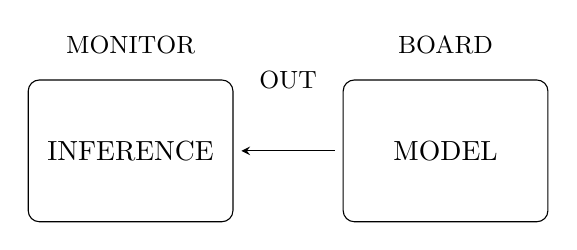
\begin{tikzpicture}[
    pinlabel/.style={font=\small},
    block/.style={draw, rounded corners,
                  minimum width=2.6cm, minimum height=1.8cm,
                  align=center},
    >=stealth
]

% --- MONITOR ---
\node[block] (monitor) at (0,0) {INFERENCE};
\node[pinlabel,anchor=south] at ([yshift=2mm]monitor.north) {MONITOR};

% --- BOARD ---
\node[block] (board) at (4,0) {MODEL};
\node[pinlabel,anchor=south] at ([yshift=2mm]board.north) {BOARD};

% OUT
\node[pinlabel] at (2,0.9) {OUT};
\draw[->] ([xshift=-0.1cm]board.west) -- ([xshift=0.1cm]monitor.east);

\end{tikzpicture}
\end{figure}

\begin{figure}[h]
\centering
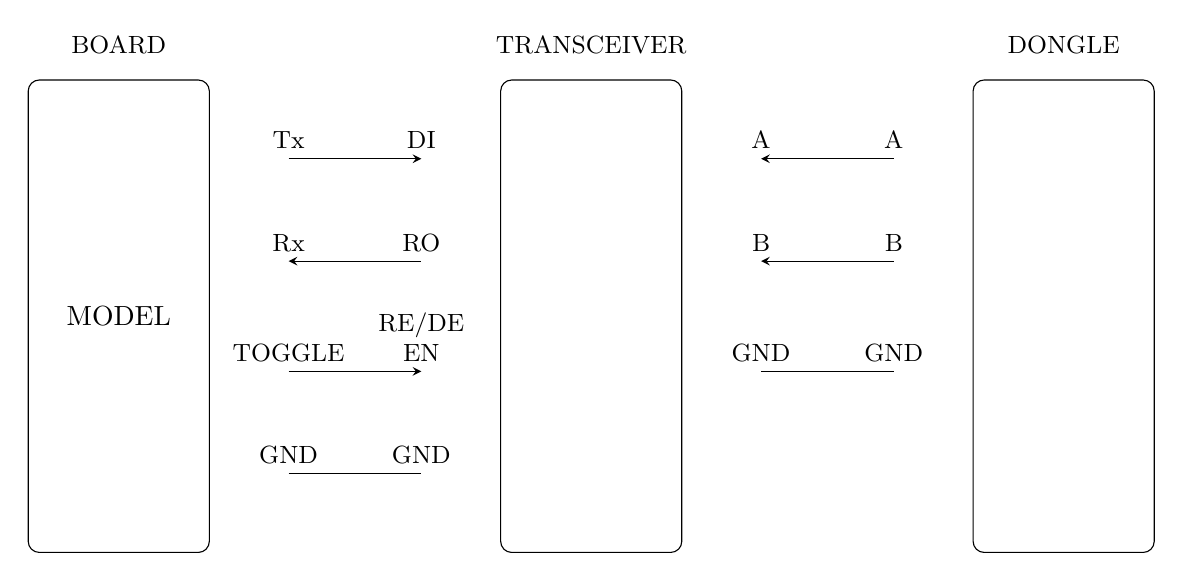
\begin{tikzpicture}[
    pinlabel/.style={font=\small},
    block/.style={draw, rounded corners,
                  minimum width=2.3cm, minimum height=6cm,
                  align=center},
    >=stealth
]

% horizontal spacing
\def\wiregap{1.0cm}

% vertical rows
\def\rowA{2cm}
\def\rowB{0.7cm}
\def\rowC{-0.7cm}
\def\rowD{-2cm}

% --- BOARD ---
\node[block] (board) at (0,0) {MODEL};
\node[pinlabel,anchor=south] at ([yshift=2mm]board.north) {BOARD};

% --- TRANSCEIVER ---
\node[block] (trans) at (6,0) {};
\node[pinlabel,anchor=south] at ([yshift=2mm]trans.north) {TRANSCEIVER};

% --- DONGLE ---
\node[block,minimum width=2.3cm] (dongle) at (12,0) {};
\node[pinlabel,anchor=south,align=center]
  at ([yshift=2mm]dongle.north) {DONGLE};

% --- BOARD → TRANSCEIVER ---
\draw[->] ([xshift=\wiregap,yshift=\rowA]board.east)
          -- ([xshift=-\wiregap,yshift=\rowA]trans.west)
          node[pinlabel,above,pos=0] {Tx}
          node[pinlabel,above,pos=1] {DI};

\draw[<-] ([xshift=\wiregap,yshift=\rowB]board.east)
          -- ([xshift=-\wiregap,yshift=\rowB]trans.west)
          node[pinlabel,above,pos=0] {Rx}
          node[pinlabel,above,pos=1] {RO};

\draw[->] ([xshift=\wiregap,yshift=\rowC]board.east)
          -- ([xshift=-\wiregap,yshift=\rowC]trans.west)
          node[pinlabel,above,pos=0] {TOGGLE}
          node[pinlabel,above,pos=1,align=center] {RE/DE\\EN};

\draw      ([xshift=\wiregap,yshift=\rowD]board.east)
          -- ([xshift=-\wiregap,yshift=\rowD]trans.west)
          node[pinlabel,above,pos=0] {GND}
          node[pinlabel,above,pos=1] {GND};

% --- TRANSCEIVER → DONGLE ---
\draw[<-] ([xshift=\wiregap,yshift=\rowA]trans.east)
          -- ([xshift=-\wiregap,yshift=\rowA]dongle.west)
          node[pinlabel,above,pos=0] {A}
          node[pinlabel,above,pos=1] {A};

\draw[<-] ([xshift=\wiregap,yshift=\rowB]trans.east)
          -- ([xshift=-\wiregap,yshift=\rowB]dongle.west)
          node[pinlabel,above,pos=0] {B}
          node[pinlabel,above,pos=1] {B};

\draw      ([xshift=\wiregap,yshift=\rowC]trans.east)
          -- ([xshift=-\wiregap,yshift=\rowC]dongle.west)
          node[pinlabel,above,pos=0] {GND}
          node[pinlabel,above,pos=1] {GND};

\end{tikzpicture}
\end{figure}

\subsubsection{Code implementation}

It is enough to configure LPUART and add RS485 transmission with guard time:

\begin{lstlisting}[language=C]
static inline void RS485_RX(void) {
    HAL_GPIO_WritePin(RS485_DE_GPIO_Port, RS485_DE_Pin, GPIO_PIN_RESET);
}

static inline void RS485_TX(void) {
    HAL_GPIO_WritePin(RS485_DE_GPIO_Port, RS485_DE_Pin, GPIO_PIN_SET);
}
\end{lstlisting}

\begin{lstlisting}[language=C]
void log_rs485(const char* s) {
    RS485_TX();
    HAL_UART_Transmit(&hlpuart1, (uint8_t*)s, strlen(s), HAL_MAX_DELAY);
    // wait for TX end so the last byte is not cut before returning to RX
    while ( HAL_UART_GET_FLAG(&hlpuart1, UART_FLAG_TC) == RESET ) {}
    RS485_RX();
}
\end{lstlisting}

Then simply route every other print to LPUART, for example:

\begin{lstlisting}[language=C]
void HAL_UART_RxCpltCallback(UART_HandleTypeDef *huart)
{
    if (huart->Instance == LPUART1) {
        char c = (char)rx_byte;
        if (c == '\n') {
            ready
        } else resets
        HAL_UART_Receive_IT(&hlpuart1, &rx_byte, 1);
    }
}
\end{lstlisting}

\subsection{On-demand standardization}

\subsubsection{Retrieval of conversion values}

Now that the wiring has been verified and everything is ready, we must first modify the \textit{MCU core} so that it can actually perform input data standardization on-board. This is necessary because, obviously, the data will be available in ``raw'' form and not pre-standardized as in the previous tests.
We therefore retrieve the \textit{standardization values} for our model. Remembering that the chosen combination is 500/0.6, we go into the folder of the experiment and open \texttt{rep\_balance\_stats.json}. We find:

\begin{verbatim}
"scaler": {
  "mean": [ . . . ],
  "scale": [ . . . ],
  ...
}
\end{verbatim}

\subsubsection{Implementation}

We therefore create two arrays \texttt{MEAN[FEAT]} and \texttt{STD[FEAT]} in x-cube-AI and use the following loop inside the \texttt{ai\_push\_line\_16} function:

\begin{lstlisting}[language=C]
int ai_push_line_of_16(const float v[FEAT]) {
    if (w_count < WIN) {
        // Standardize each feature: z = (x - μ) / σ
        for (int i = 0; i < FEAT; i++) {
            window[w_count][i] = (v[i] - MEAN[i]) / STD[i];
        }
        w_count++;
    }
    return 0;
}
\end{lstlisting}

\subsubsection{Observations}

At this point we only need to confirm the correctness of the code. We compare the windows standardized by the MCU and those produced by the external standardizer (the previous Python script) that generated the ready-to-use window. The code is identical. In fact, the output produced by the MCU is the same. We use the same \texttt{invio.py} as before but with the new window.

\textbf{IMPORTANT NOTE}:  
Previously, we had extracted a window \emph{after} applying the standard scaler. For precision reasons, we created a script that generates both a RAW window and the corresponding Standard window together, so that we can operate on both versions at once. In this way we have a complete tester; otherwise we would have had to invert the previously standardized window, again risking precision loss.

\begin{lstlisting}

[MODE] Modbus RTU - Listening on RS-485...
\end{lstlisting}

\section{Section 7 -- Modbus RTU Implementation}

\begin{table}[h]
\centering
\begin{tabular}{c c c c c c}
\multicolumn{6}{c}{\textbf{Modbus RTU Frame Format}}\\[4pt]
\textbf{Start} & \textbf{Address} & \textbf{Function} & \textbf{Data} & \textbf{CRC} & \textbf{End} \\
$\geq$3.5 char & 8 bit & 8 bit & $N \cdot 8$ bit & 16 bits & $\geq$3.5 char \\
\\
\multicolumn{6}{c}{\textbf{Modbus ASCII Frame Format}}\\[4pt]
\textbf{Start} & \textbf{Address} & \textbf{Function} & \textbf{Data} & \textbf{LRC} & \textbf{End} \\
; & 2 chars & 2 chars & $N \cdot 1$ chars & 2 chars & CR, LF \\
\end{tabular}
\end{table}

\subsection{Theory and initial scheme}

The final and important step is to adopt a common \textit{industrial standard} (and the one used by the Bonfiglioli sensor) for reading the sensor data. So far, we have used a simple Python file sending ASCII.  
Let us start by clarifying that Bonfiglioli has two z-sensors acting as \emph{slaves} connected to a master that reads their values. We will have to connect the MCU to the same bus (as an \textit{additional slave}) and sniff the values, then continue with the pipeline. Note that the standard is binary, with the following layout:

\begin{verbatim}
[ADDR][FUNC][LEN][PAYLOAD][CRC_LOW][CRC_HIGH]
\end{verbatim}

\begin{itemize}
    \item ADDR = slave address (1 byte)
    \item FUNC = function code (1 byte)
    \item LEN = payload length (1 byte)
    \item PAYLOAD = actual data
    \item CRC16 = final checksum (2 bytes, little-endian)
\end{itemize}

We will use, in order:

\begin{itemize}
    \item 0x01 (arbitrary slave address)
    \item 0x03 (Read Holding Registers)
    \item 0x40 (64 in decimal, 16 float values (4 bytes each) $\rightarrow$ 64 bytes)
    \item 64 bytes written one by one in big-endian order (most significant byte first)
    \item Standard CRC L/H for checksum
\end{itemize}

Note: This payload is custom. Modbus registers are 16-bit (2 bytes); Modbus knows nothing about floats. Therefore each float will be split into \textbf{two separate 16-bit registers} so that it can be transmitted. We do not know exactly why the CSV data are all floats, even though standard Modbus RTU is used.

\textbf{OPEN QUESTION 1 $\rightarrow$ HOW do they send these floats on their side (if they do send floats)? Custom mapping?}

\subsubsection{Master simulator}

Once the semantics of the frame have been fixed, we implement them in a script that simulates a master \textit{publishing those values}, accessible via the TX/RX link.

\begin{lstlisting}[language=Python]
def modbus_crc16(data):
    """Compute Modbus CRC16 (polynomial 0xA001)."""
    crc = 0xFFFF
    for byte in data & _ in range:
                crc >>= 1
    ...

def build_modbus_frame(slave_addr, function_code, float_values):
    
    frame.append(slave_addr)
    for value in float_values:
        frame.extend(struct.pack('>f', value))  # '>f' = big-endian float
    crc = modbus_crc16(frame)
    frame.append(crc & 0xFF)         # CRC Low
    frame.append((crc >> 8) & 0xFF)  # CRC High
\end{lstlisting}

\subsubsection{Continuous sending}

Inside a \texttt{while True} we encapsulate the send logic, followed by a final \texttt{sleep} after the log (not shown but present right after):

\begin{lstlisting}[language=Python]
for idx, row in df.iterrows():
    # Extract , Build Modbus RTU frame Compute CRC for verification and send frame
    ser.write(frame)
    frame_count += 1
\end{lstlisting}

\subsection{Data reception on the MCU side}

\subsubsection{Callback}

First we prepare the MCU to run the following callback in \texttt{main.c} on each received byte:

\begin{lstlisting}[language=C]
void HAL_UART_RxCpltCallback(UART_HandleTypeDef *huart) {
    if (huart->Instance == LPUART1) {
        if (protocol_mode == PROTOCOL_MODE_MODBUS) {
            // NO LOGS HERE, ONLY NECESSARY OPERATIONS
            uint32_t now = HAL_GetTick();
            modbus_rx_buffer|timestamp|head|lastime
        }
    }
}
\end{lstlisting}

In particular, at each interrupt it:

\begin{itemize}
    \item stores the byte in \texttt{modbus\_rx\_buffer[]} (circular buffer),
    \item also stores the timestamp in \texttt{modbus\_rx\_timestamps[]} (same circular indexing),
    \item advances the index of \texttt{modbus\_rx\_buffer[]} (the same used for \texttt{modbus\_rx\_timestamps[]}),
    \item immediately re-arms \texttt{HAL\_UART\_Receive\_IT} waiting for the next interrupt.
\end{itemize}

\textbf{OPEN QUESTION 2 $\rightarrow$} the index increases linearly and could eventually overflow the underlying \texttt{uint32\_t} if it were never reset. This should be adjusted.

\subsubsection{Buffer consumption}

Then, in the main loop (daemon) we consume the two buffers with a proximity logic: as long as the tail of the main buffer does not coincide with the head, there are bytes in between to process (and therefore also in \texttt{timestamps}, which is indexed with the same variable).

To do this, we create two new modules to keep the code organized clearly: \texttt{app\_x-cube-ai.c/h} in \texttt{Core/Inc} (header) and \texttt{Core/Src} (source).

\subsection{Support modules for Modbus RTU processing}

The \texttt{.c} file follows a common community pattern, but needs some functions implemented ad hoc:

\begin{itemize}
    \item \texttt{modbus\_process\_byte()} : takes one byte at a time with its timestamp, recognizes the binary sequence defined earlier and returns 1 if the frame is complete (so the payload can be extracted by other functions)
    \item \texttt{modbus\_get\_frame()} : copies out the recognized frame
    \item \texttt{modbus\_extract\_float32()} : extracts the payload of 16 floats
\end{itemize}

Note: each function is obviously non-blocking, but skips subsequent blocks and returns to the same point (polling) until the condition is met.

\textbf{OPEN QUESTION 3 $\rightarrow$} we are effectively wrapping Modbus; normally one would also implement the register logic and CRC handling in a more complete way.

\subsubsection{\texttt{modbus\_process\_byte}}

\begin{center}
    \textit{See the GitHub}
\end{center}


\subsubsection{\texttt{modbus\_get\_frame}}

\begin{center}
    \textit{See the GitHub}
\end{center}

\subsubsection{\texttt{modbus\_extract\_float32}}

\begin{center}
    \textit{See the GitHub}
\end{center}

\subsection{Main loop (daemon in \texttt{main.c})}

Here, as mentioned earlier, we use the functions just implemented.

\subsubsection{Main loop}

\begin{lstlisting}[language=C]
while (1) {

    // === MODBUS RTU ===
    if (protocol_mode == PROTOCOL_MODE_MODBUS) {
        // Process bytes
        while (modbus_rx_tail != modbus_rx_head) {
            squeeze
            if (modbus_process_byte(&modbus_buf, byte, timestamp)) {
                // Frame completed! Filter & Push:
                ai_push_line_of_16(raw_features);
                log_vcp(line);
                        }
                    }
                }
            }
        }
    }
}
\end{lstlisting}

\begin{itemize}
    \item We consume bytes from the circular buffer via \texttt{modbus\_process\_byte()} and, as soon as the function returns 1, the sequence of bytes forms a meaningful frame.
    \item We copy the valid frame with \texttt{modbus\_get\_frame()} (and also check that the frame is valid).
    \item We extract the payload with \texttt{modbus\_extract\_float32()}.
\end{itemize}

\subsubsection{Push}

At this point, we can push the data: we call \texttt{ai\_push\_line\_of\_16()} passing the payload (a new row). The x-cube-AI flow is then invoked. Recalling the overall logic:

\begin{itemize}
    \item The incoming row is parsed and, at the same time, passed to a function that in turn calls a (custom) function inside x-cube-AI that pushes the row inside a window. When the global ``window'' is ready, a global flag is set to 1.
    \item The standard x-cube-AI processing is called, which checks the flag: if the window is ready, it standardizes and feeds the model.
\end{itemize}

This last part is omitted here because it was already shown earlier. The pipeline is therefore complete.

\subsection{Functional testing}

We flash the above firmware onto the MCU, and we open the debug port:

\begin{verbatim}
screen /dev/ttyACM0 115200
\end{verbatim}

Then we send:

\begin{verbatim}
python modbus_simulator.py win_raw.csv 2.0
\end{verbatim}

The inference is \textbf{correctly} displayed on the console:

\begin{lstlisting}[language=bash]

[TX #0030] Row 30/30 | Frame: 69 bytes | CRC: 0x2c16  ✅
Sample: [3.638, -0.246, 0.915, ..., 52.750]
Hex: 01 03 40 6b d8 0e 44 0b ...

[INFO] End of iteration 1. Restarting...
-------------------------------------------------------
...
[MODBUS] Frame OK #29 (len=64)
[AI] *** WINDOW 30/30 COMPLETE -> INFERENCE ***
[AI] Inference done. Q->F:
0.104 -0.104 0.677 -0.156 0.989 2.290 0.989 0.521 0.416 0.104 ...
...

\end{lstlisting}

\subsection{Errors during deployment}

To avoid confusion, we briefly list the main errors encountered before reaching the correct pipeline:

\begin{itemize}
    \item Use of model 2000/0.5 both as the deployed network and in the standardization parameters. Result: \textbf{confused} benchmarking.
    \item Window already standardized and then standardized again (old code remained). Same effect.
    \item Logging inside a callback. Again, a typical mistake that causes lost data on the receive buffer (even if the transmission is constant).
    \item Python packed data in \textit{little-endian}, but the MCU expected big-endian. Classic error: the end of the window did not match.
\end{itemize}

\begin{center}
    \textbf{Final note: the models have the same size.}
\end{center}

\section{Questions}

\begin{itemize}
    \item[] $\rightarrow$ QUESTION: WE INCLUDED THE TAILS IN TRAINING. IS THERE A RISK OF NOT RECOGNIZING THEM?
    \item[] \texttt{trainingincluselecode-colonne16}
    \item[] Training done assuming 80\% reliability.
    \item[] Modbus addresses.
\end{itemize}

\section*{Important final notes}

\begin{itemize}
    \item This Board has an ICache in addition to the prefetch cache, which is worth enabling from the beginning: this can be configured from the System Core so that its \texttt{init()} is called at the start of the code. For this project it is convenient to use the 2-way (column) configuration, because we will not be in a purely linear coding situation but will have multiple libraries + loops (+overhead but more reliable under cache misses).
    \item Be careful, in the \texttt{while(1)}, to write the code in the correct user regions: it is not enough to place it inside the braces. At each save, in fact, any code regenerated outside the \texttt{USER CODE BEGIN/END} comments risks being overwritten.
    \item The reset button restarts \texttt{main} from scratch, clearing RAM but not FLASH. This means that reset can be used safely whenever we need to clear Cache/RAM, without worrying about losing any persistent data.
\end{itemize}

\section*{Notes}

The CNN architecture was chosen instead of a Spiking Neural Network (SpikeNN) for practical reasons. Although SpikeNN is more recent, potentially more efficient and with lower resource consumption, its training is demanding and difficult to get right in practice.

% \section*{References}

% \begin{itemize}
%     \item Hochreiter, S.; Schmidhuber, J. (1997). Long Short-Term Memory. Neural Computation, 9(8), 1735–1780.
%     \item Malhotra, P.; Ramakrishnan, A.; Anand, G.; Vig, L.; Agarwal, P.; Shroff, G. (2016). LSTM-based Encoder–Decoder for Multi-sensor Anomaly Detection. arXiv:1607.00148.
%     \item Bai, S.; Kolter, J. Z.; Koltun, V. (2018). An Empirical Evaluation of Generic Convolutional and Recurrent Networks for Sequence Modeling. arXiv:1803.01271.
%     \item Zhang, C.; Song, D.; Chen, Y.; et al. (2019). MSCRED: A Deep Neural Network for Unsupervised Anomaly Detection and Diagnosis in Multivariate Time Series. AAAI 2019.
%     \item Zong, B.; Song, Q.; Min, M. R.; et al. (2018). Deep Autoencoding Gaussian Mixture Model for Unsupervised Anomaly Detection. ICLR 2018.
%     \item Su, Y.; Zhao, Y.; Niu, C.; et al. (2019). Robust Anomaly Detection for Multivariate Time Series through Stochastic RNN (OmniAnomaly). KDD 2019.
%     \item Xu, H.; Chen, W.; Zhao, N.; et al. (2018). Unsupervised Anomaly Detection via Variational Auto-Encoder for Seasonal KPIs in Web Applications (Donut). WWW 2018.
%     \item Bañós, O.; Gálvez, J.-M.; Damas, M.; Pomares, H.; Rojas, I. (2014). Window Size Impact in Human Activity Recognition. Sensors, 14(4), 6474–6499.
%     \item Ronao, C. A.; Cho, S.-B. (2016). Human Activity Recognition with Smartphone Sensors Using Deep Learning Neural Networks. Expert Systems with Applications, 59, 235–244.
%     \item Dehghani, A.; Nambiar, R.; Sharma, R.; et al. (2019). A Quantitative Comparison of Overlapping and Non-Overlapping Sliding Windows for HAR Using Inertial Sensors. Sensors, 19(22), 5026.
%     \item Randall, R. B.; Antoni, J. (2011). Rolling Element Bearing Diagnostics—A Tutorial. Mechanical Systems and Signal Processing, 25(2), 485–520.
%     \item Mohd Ghazali, M. H.; Rahiman, W. (2021). Vibration Analysis for Machine Monitoring and Diagnosis: A Systematic Review. Shock and Vibration, Article ID 9469318.
% \end{itemize}
